\documentclass[11pt]{article}

% AMS Packages
\usepackage{amsmath} 
\usepackage{amssymb} 
\usepackage{amsthm}
% Page dimensions
\usepackage[margin=0.9in]{geometry}
% Images
\usepackage[pdftex]{graphicx} 
% Enumerate package
\usepackage{enumitem} 
\usepackage{array} 
% Fancify pages
\usepackage{fancyhdr} 
% Convert captions on figures to bold font
\usepackage[labelfont=bf,textfont=md]{caption}
% Time New Roman font
\usepackage{times}
% package to set line spacings
\usepackage{setspace} 
% SI Units in math type
\usepackage{siunitx}
\usepackage{textcomp} 
% Change sizes of sections
\usepackage{titlesec}
\titleformat{\section}{\normalfont\large\bfseries}{\thesection}{1em}{}
\titleformat{\subsection}{\normalfont\bfseries}{\thesubsection}{1em}{}
\titleformat{\subsubsection}{\normalfont\small\bfseries}{\thesubsubsection}{1em}{}
% Declare useful math operators
\DeclareMathOperator*{\argmin}{arg\,min}
\DeclareMathOperator*{\plim}{plim}
\DeclareMathOperator{\Tr}{Tr}


\begin{document}
\section{UoI$_\text{Lasso}$ Stability Selection}
	Union of Intersections (UoI) enforces a strict intersection of supports over bootstraps in its traditional implementation. To be clear, suppose we have $B_1$ bootstraps in the selection module; then, a feature must be selected in all $B_1$ bootstraps (of $\lambda_i$) to be passed along in the proposed support for the regularization strength $\lambda_i$. We can relax this assumption by only requiring that a feature appear in some fraction $f_s$ of the bootstraps, i.e. it appears in $f_s B_1$ selection bootstraps where $0 < f_s \leq 1$. Choosing $f_s$ wisely can result in a reduction of false negatives since we are softening the requirements for a feature to be selected.
	
	We have a problem, though: we must choose $f_s$ wisely. In effect, it becomes another hyperparameter in the optimization procedure. One approach is to let the UoI algorithm choose $f_s$ in a similar fashion that it chooses the regularization strength $\lambda$. Traditional UoI would pass $N_{\lambda}$ supports to the estimation module, where $N_{\lambda}$ is the number of $\lambda$ values. We could instead pass $N_{\lambda} \times N_{f_s}$ supports to the estimation module, where we apply $N_{f_s}$ selection thresholds to each of the original $N_{\lambda}$ supports. This serves as the natural extension of UoI to the case of multiple hyperparameters.
	
	Stability selection would be particularly useful in the case of collinear features. Two highly collinear features might be selected in different supports in lieu of each other, diluting their appearance in the supports of the $B_1$ bootstraps. In a traditional UoI$_{\text{Lasso}}$, neither would be selected. Thus, relaxing the selection criteria might allow both features to be selected. If UoI treats the selection threshold as a hyperparameter, it's possible for it to find the best selection threshold based on the predictive quality of the model.

\section{Implementation}
	Our implementation is as follows. UoI$_{\text{Lasso}}$ accepts (among others) two hyperparameters: $N_{\lambda}$ (number of $\lambda$ hyperparameters) and $L_{f_s}$ (lower bound for selection threshold). The sweep over $\lambda$ values is performed in the traditional fashion, with a coarse sweep followed by a dense sweep. Then, the sweep over selection thresholds is chosen by $\left[L_{f_s}, 1.0\right]$, with corresponding bootstrap requirements of $\left[L_{f_s}\cdot B_1, B_1\right]$. The number of selection thresholds chosen from the range $\left[L_{f_s}\cdot B_1, B_1\right]$ is set by default to be large enough that all possible bootstrap numbers are included. 
	
	Thus, UoI$_{\text{Lasso}}$ will perform the estimation module using $B_2$ bootstraps over $N_{\lambda}\times N_{f_s}$ supports. Importantly, we will use BIC to evaluate and choose the final features in the estimation module.
	
\section{Experiment 1}
	Our first experiment considers how the selection threshold aids in cases of collinear features. Our toy dataset consists of a design matrix $\mathbf{X}$ with $M$ features. These features are divided into groups of 5, and there is a covariance structure assigned to each group. Thus, the covariance matrix across the entire dataset takes on a block-diagonal form:
	\begin{align}
		\boldsymbol{\Sigma} &= \left(
			\begin{array}{cccc}
			\mathbf{B} &	0 & \cdots  &	0\\
				0			 & \mathbf{B} & \cdots & 0 \\
			\vdots		 & 	\vdots			& \ddots & 0 \\
			0 & 0 & 0  & \mathbf{B}
			\end{array}
		\right)
	\end{align}
	where $\mathbf{B}$ is the covariance matrix for each group of five features. 
	
	In this experiment, we considered 25 features divided into groups of 5. The block covariance structure $\mathbf{B}$ assigned uniform correlations among features within each group. Furthermore, for each run, the correlation was the same across all groups: this value was $r$. We then formed a response vector as follows:
	\begin{align}
		y &= \mathbf{X}\boldsymbol{\beta} + \epsilon
	\end{align}
	where $\boldsymbol{\beta}$ were just drawn from a uniform distribution, and the noise term was standard normal: $\epsilon \sim \mathcal{N}(0, \sigma^2)$, with variance set to enforce an inverse signal-to-noise ratio of $\kappa=0.3$. Lastly, the $\boldsymbol{\beta}$ consisted of only non-zero parameters, so we were only concerned with reducing false negatives.
	
	We considered a range of correlations $r\in \left\{0, \ldots, 1.0\right\}$ built into the block covariance $\mathbf{B}$. Thus, for $r=1.0$, our dataset consisted of 5 groups of perfectly (but separately) correlated features. We ran UoI$_{\text{Lasso}}$ on data generated from 50 models with various lower selection thresholds $L_{f_s}$. Our results are shown in Figure \ref{fig:fn-vs-thres}. 	In addition, explained variances are depicted in Figure \ref{fig:r2-vs-thres}.
	\begin{figure}[ht]
		\centering
		\scalebox{0.32}{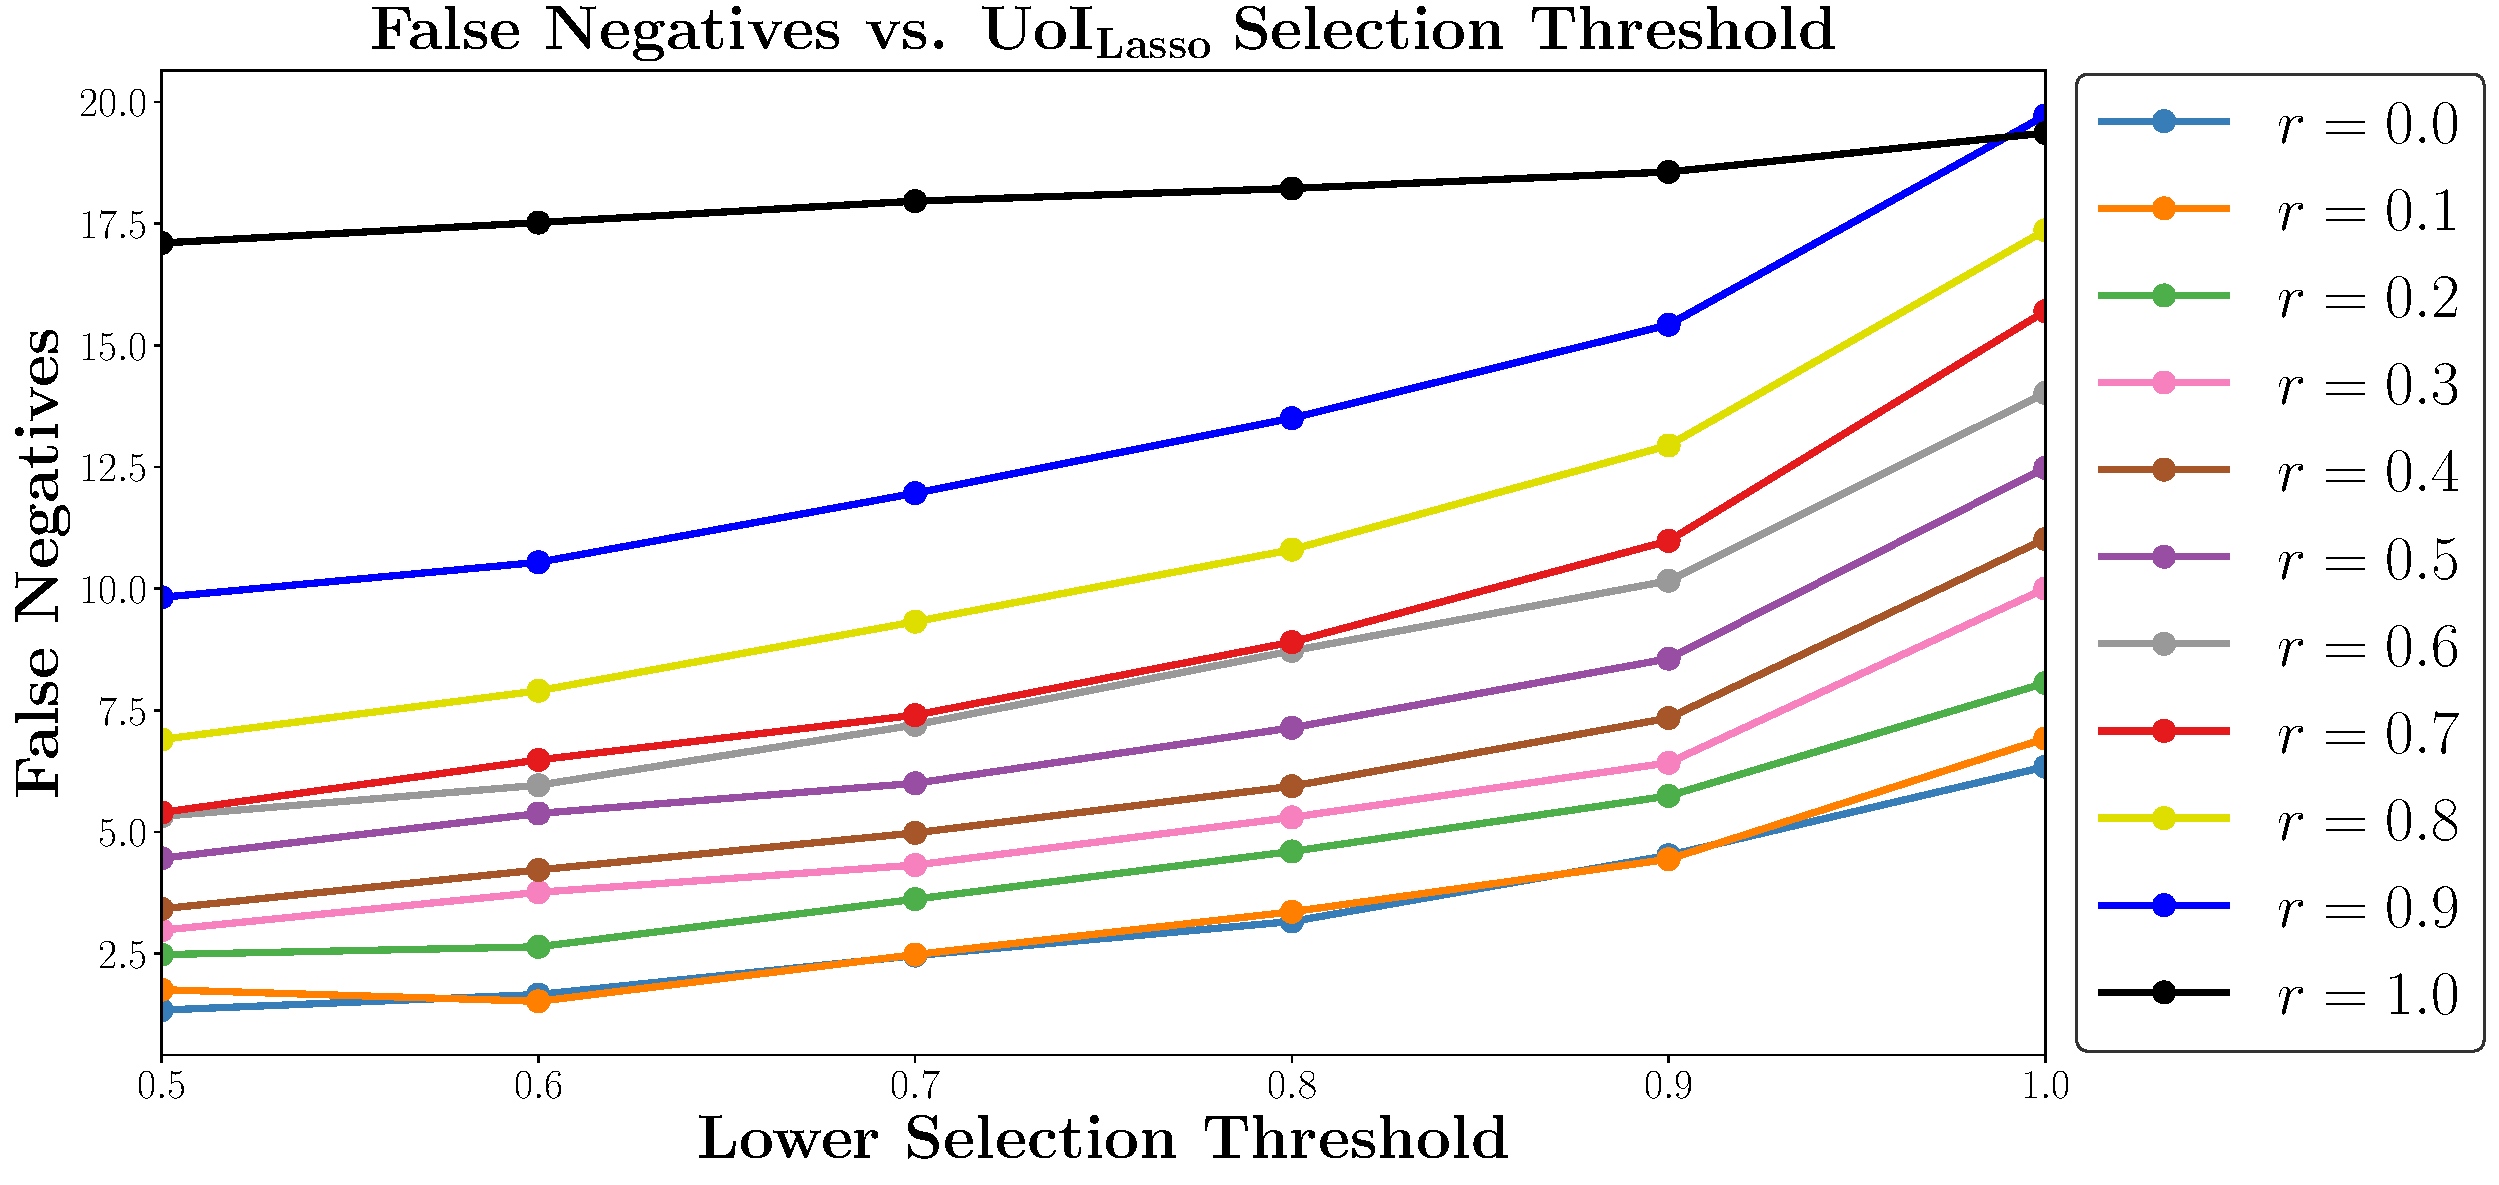
\includegraphics{img/fn_vs_lower_threshold.pdf}}
		\caption{False negatives vs. Lower selection threshold. Depicted are averages over 50 separate models. As we decrease the selection threshold, we select more variables and therefore observe fewer false negatives. Traditional UoI$_{\text{Lasso}}$ is given by $L_{f_s} = 1.0$ on the right hand side. For $r=1.0$, we see 20 false negatives, which makes sense: UoI$_{\text{Lasso}}$ will only select one variable among each of the five groups (setting the remaining 20 to zero).}
		\label{fig:fn-vs-thres}
	\end{figure}
	\begin{figure}[ht]
		\centering
		\scalebox{0.32}{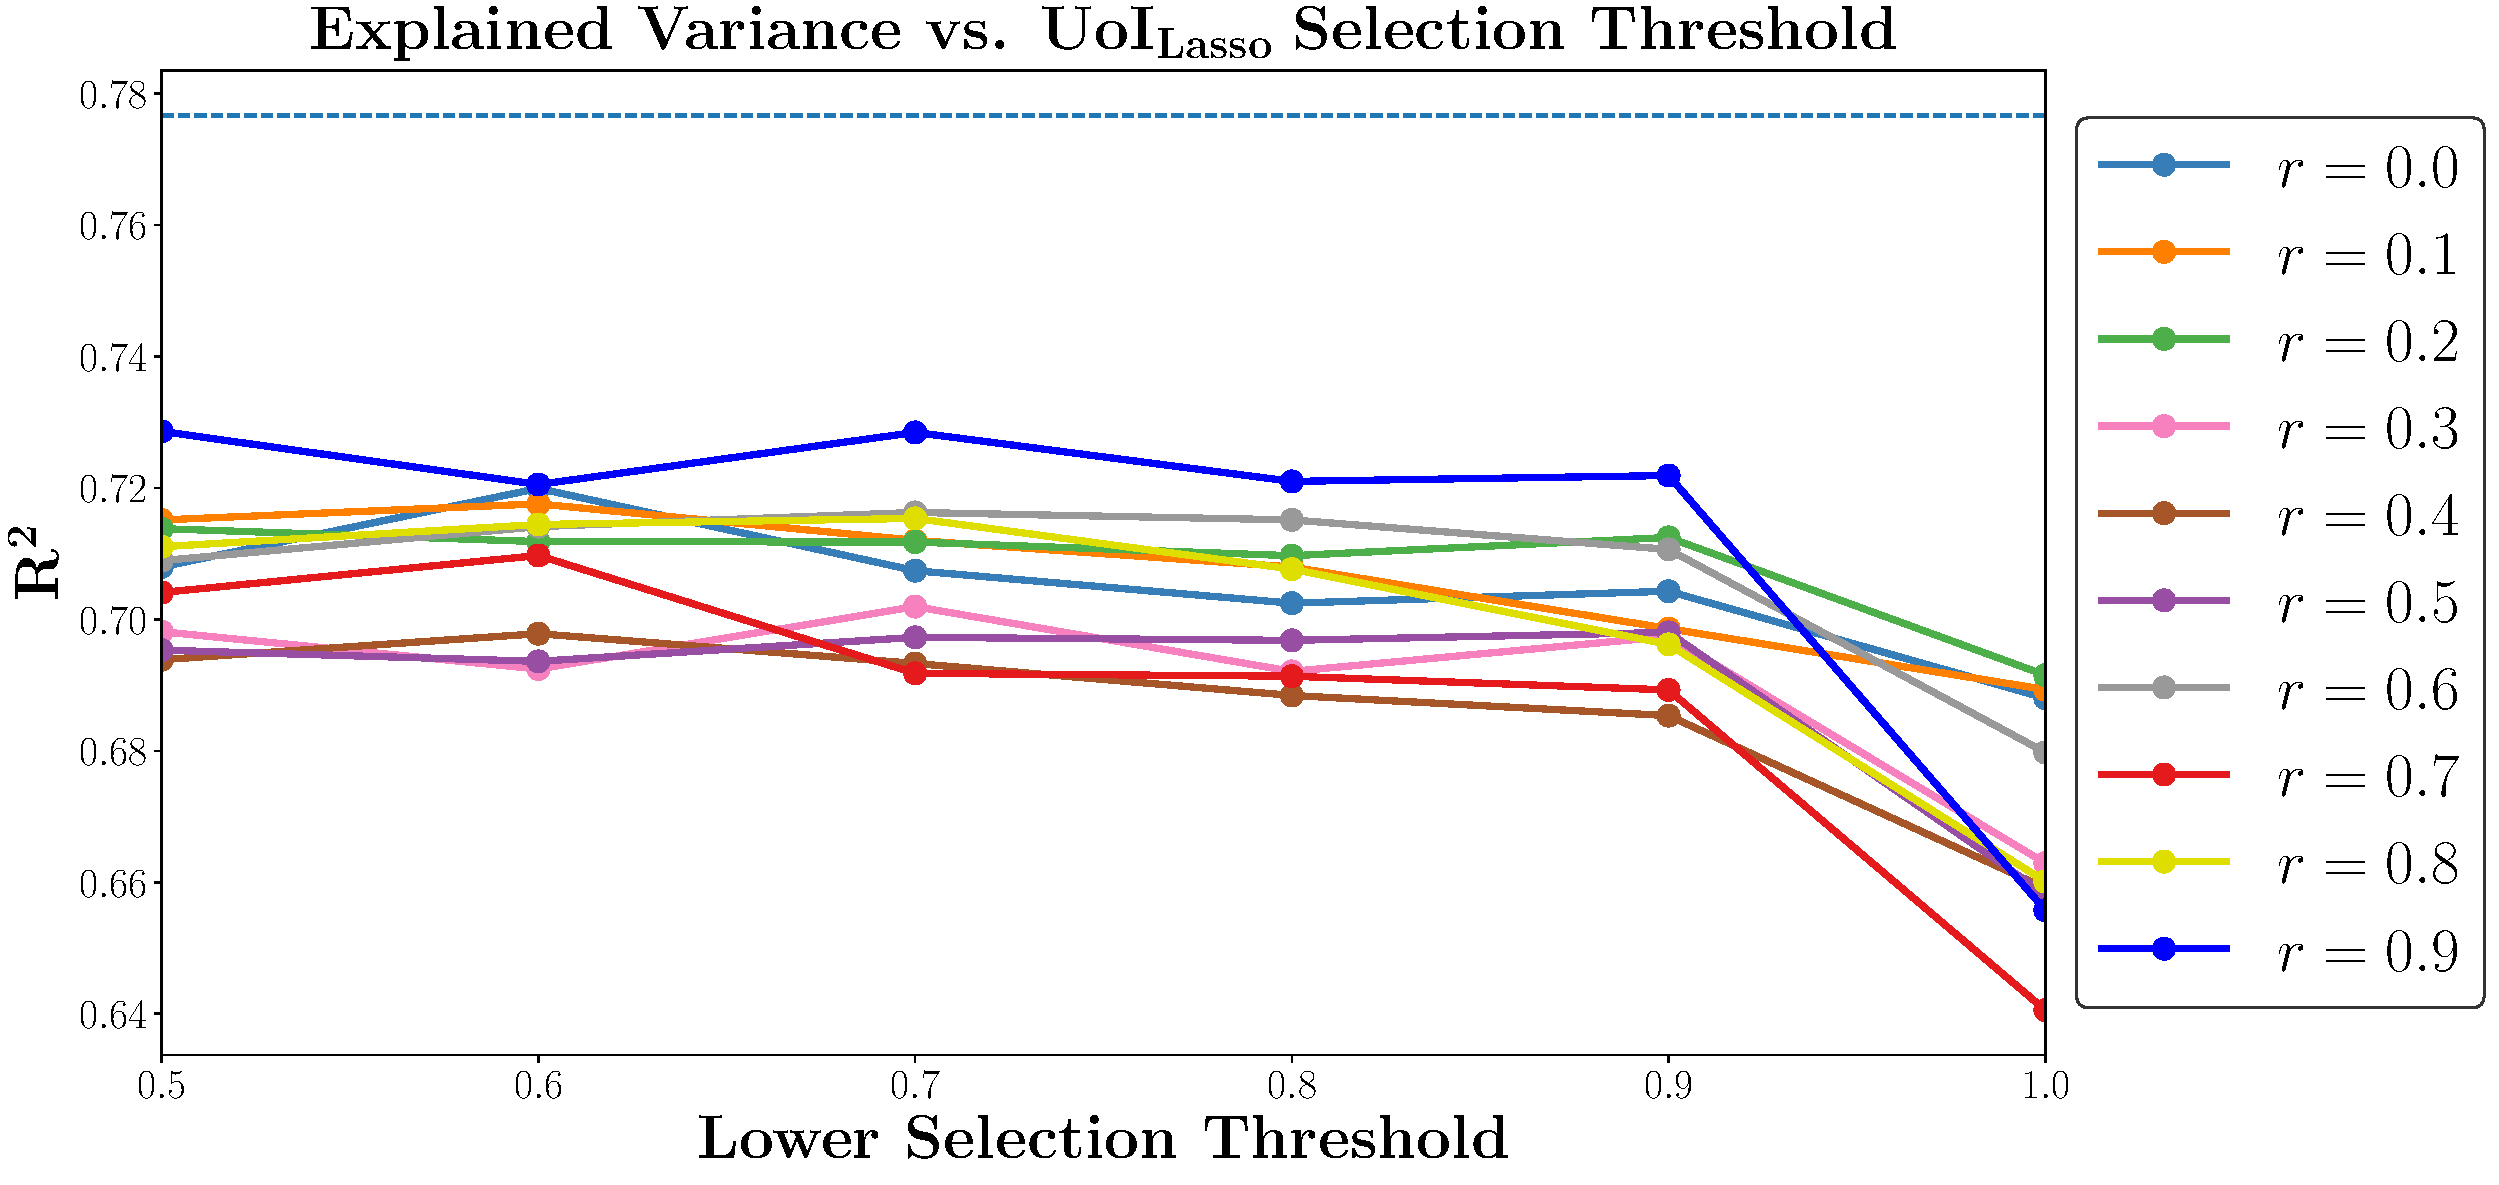
\includegraphics{img/r2_vs_lower_threshold.pdf}}
		\caption{Median explained variance over various lower selection thresholds. There is generally an increase in $R^2$ as $L_{f_s}$ is decreased. The dashed blue line indicates the median performance by the true parameters. Lastly, we did not include $r=1.0$ since the $R^2$ was poor.}
		\label{fig:r2-vs-thres}
	\end{figure}

\section{Experiment 2}
For the second experiment, we varied the sparsity of the true parameters. This allowed there to be both false positives and false negatives. For example, consider a model with 50 features divided into 5 groups of 10 and a sparsity of $s=0.4$. The sparsity was enforced in such a way that each group had $10 \times 0.4 = 4$ non-zero parameters. 
False positives and false negatives are shown below.
\begin{figure}[ht]
	\centering
	\scalebox{0.27}{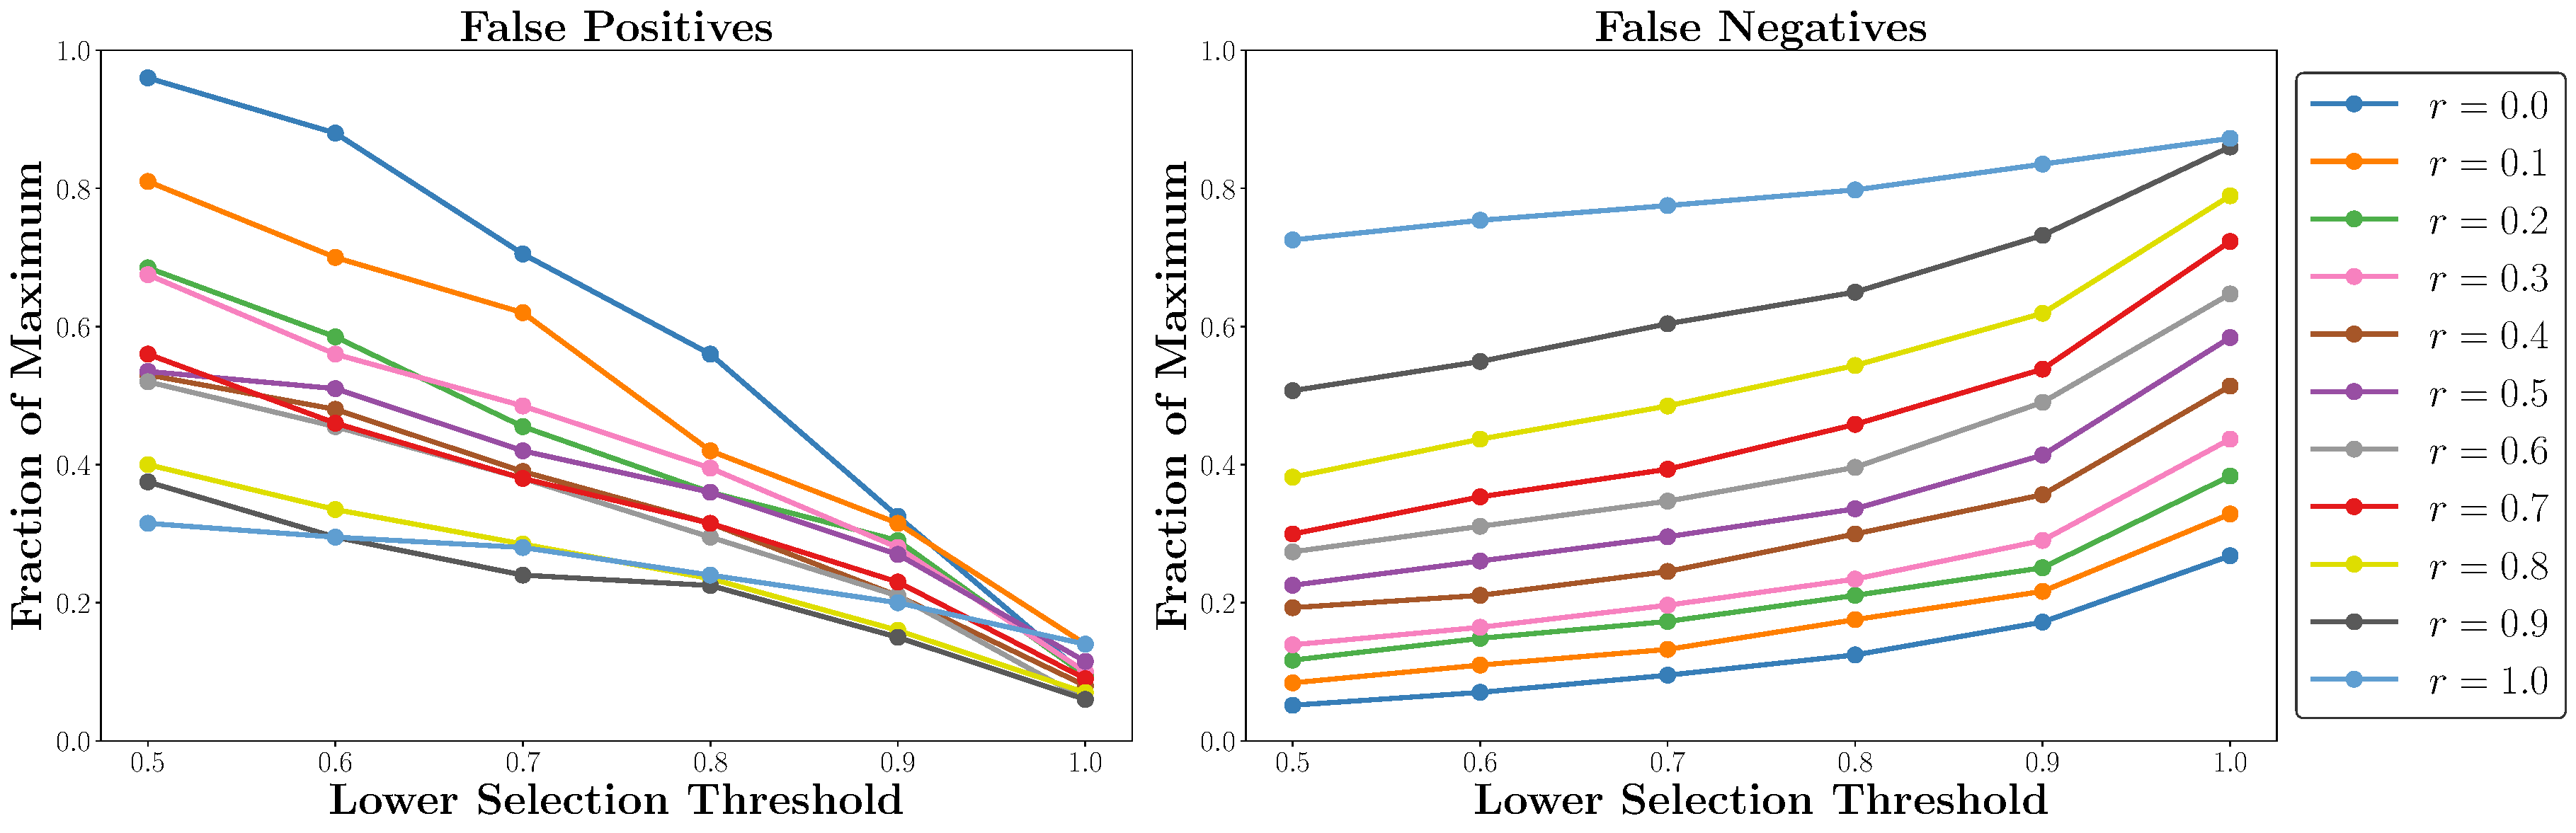
\includegraphics{img/exp2-09.pdf}}
\end{figure}
\begin{figure}[ht]
	\centering
	\scalebox{0.27}{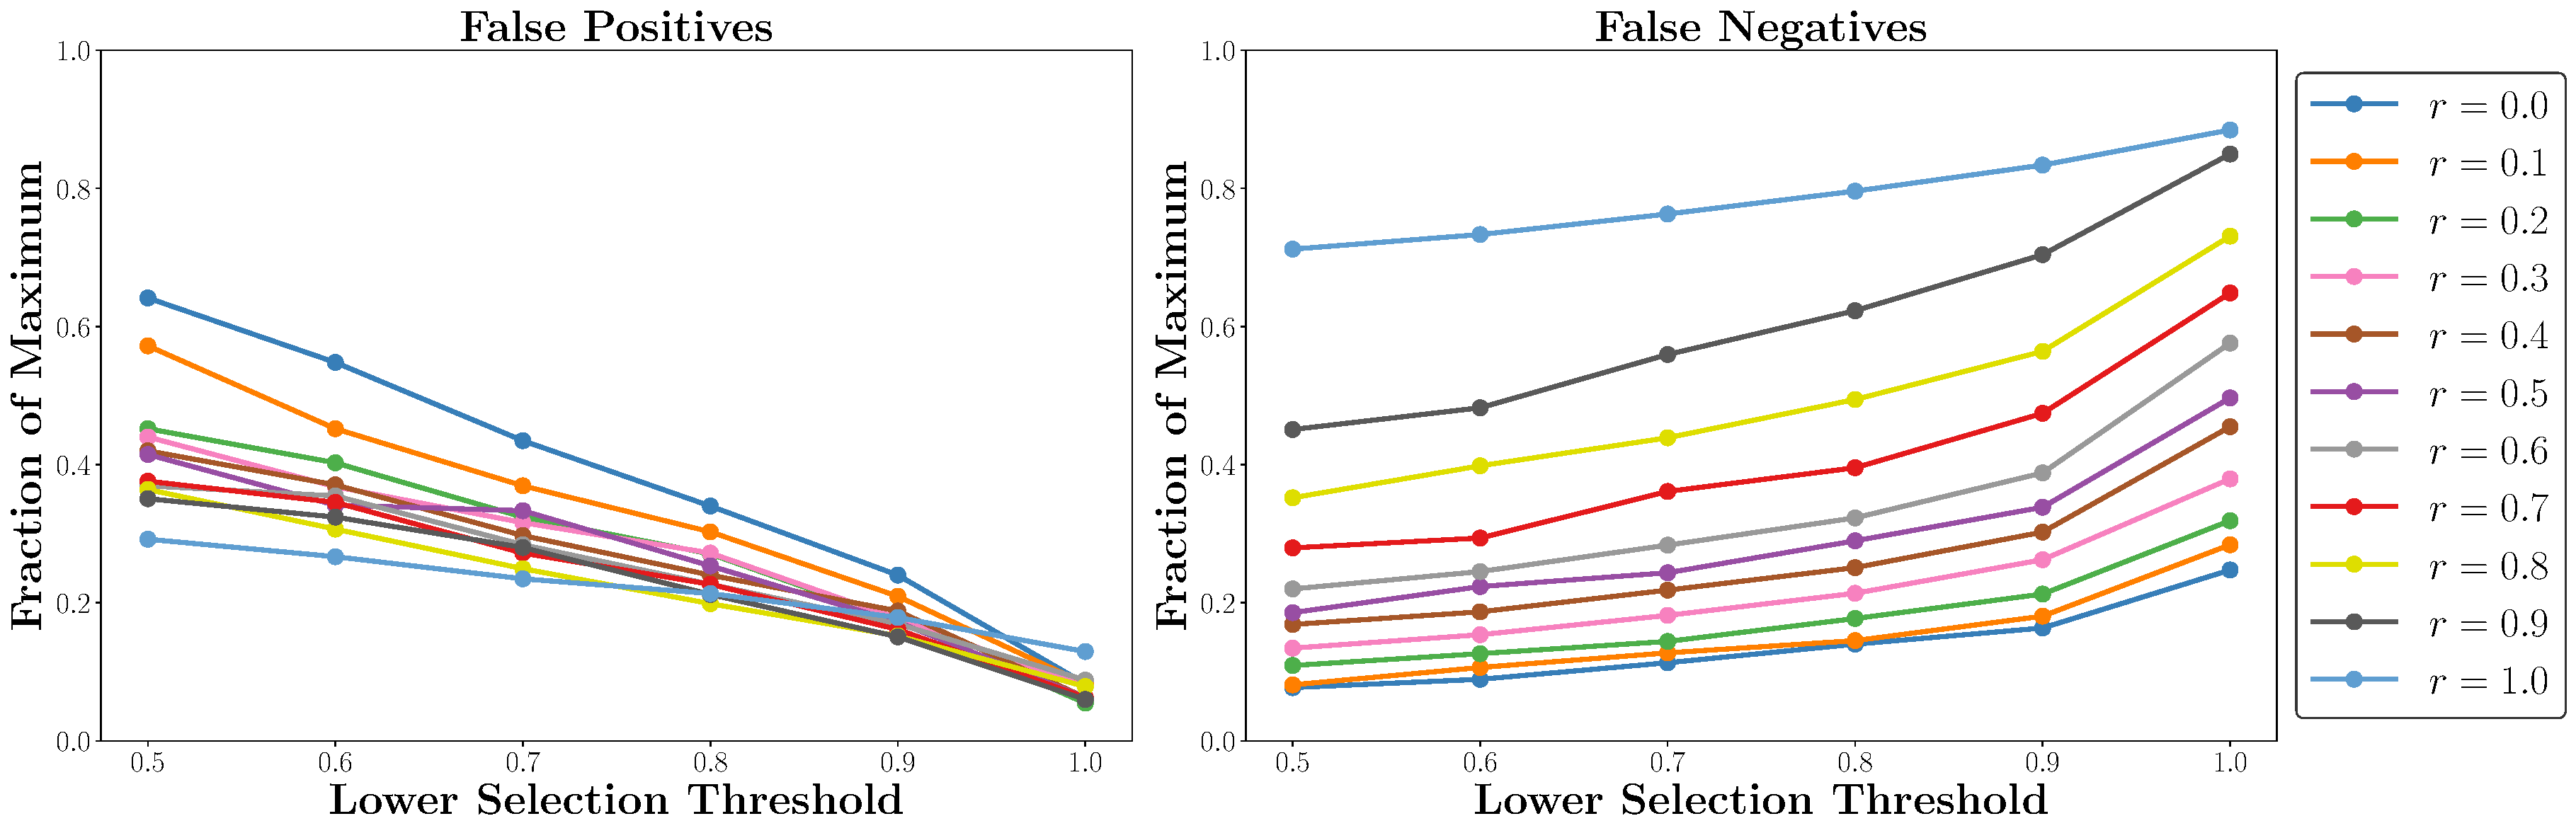
\includegraphics{img/exp2-07.pdf}}
\end{figure}
\begin{figure}[ht]
	\centering
	\scalebox{0.27}{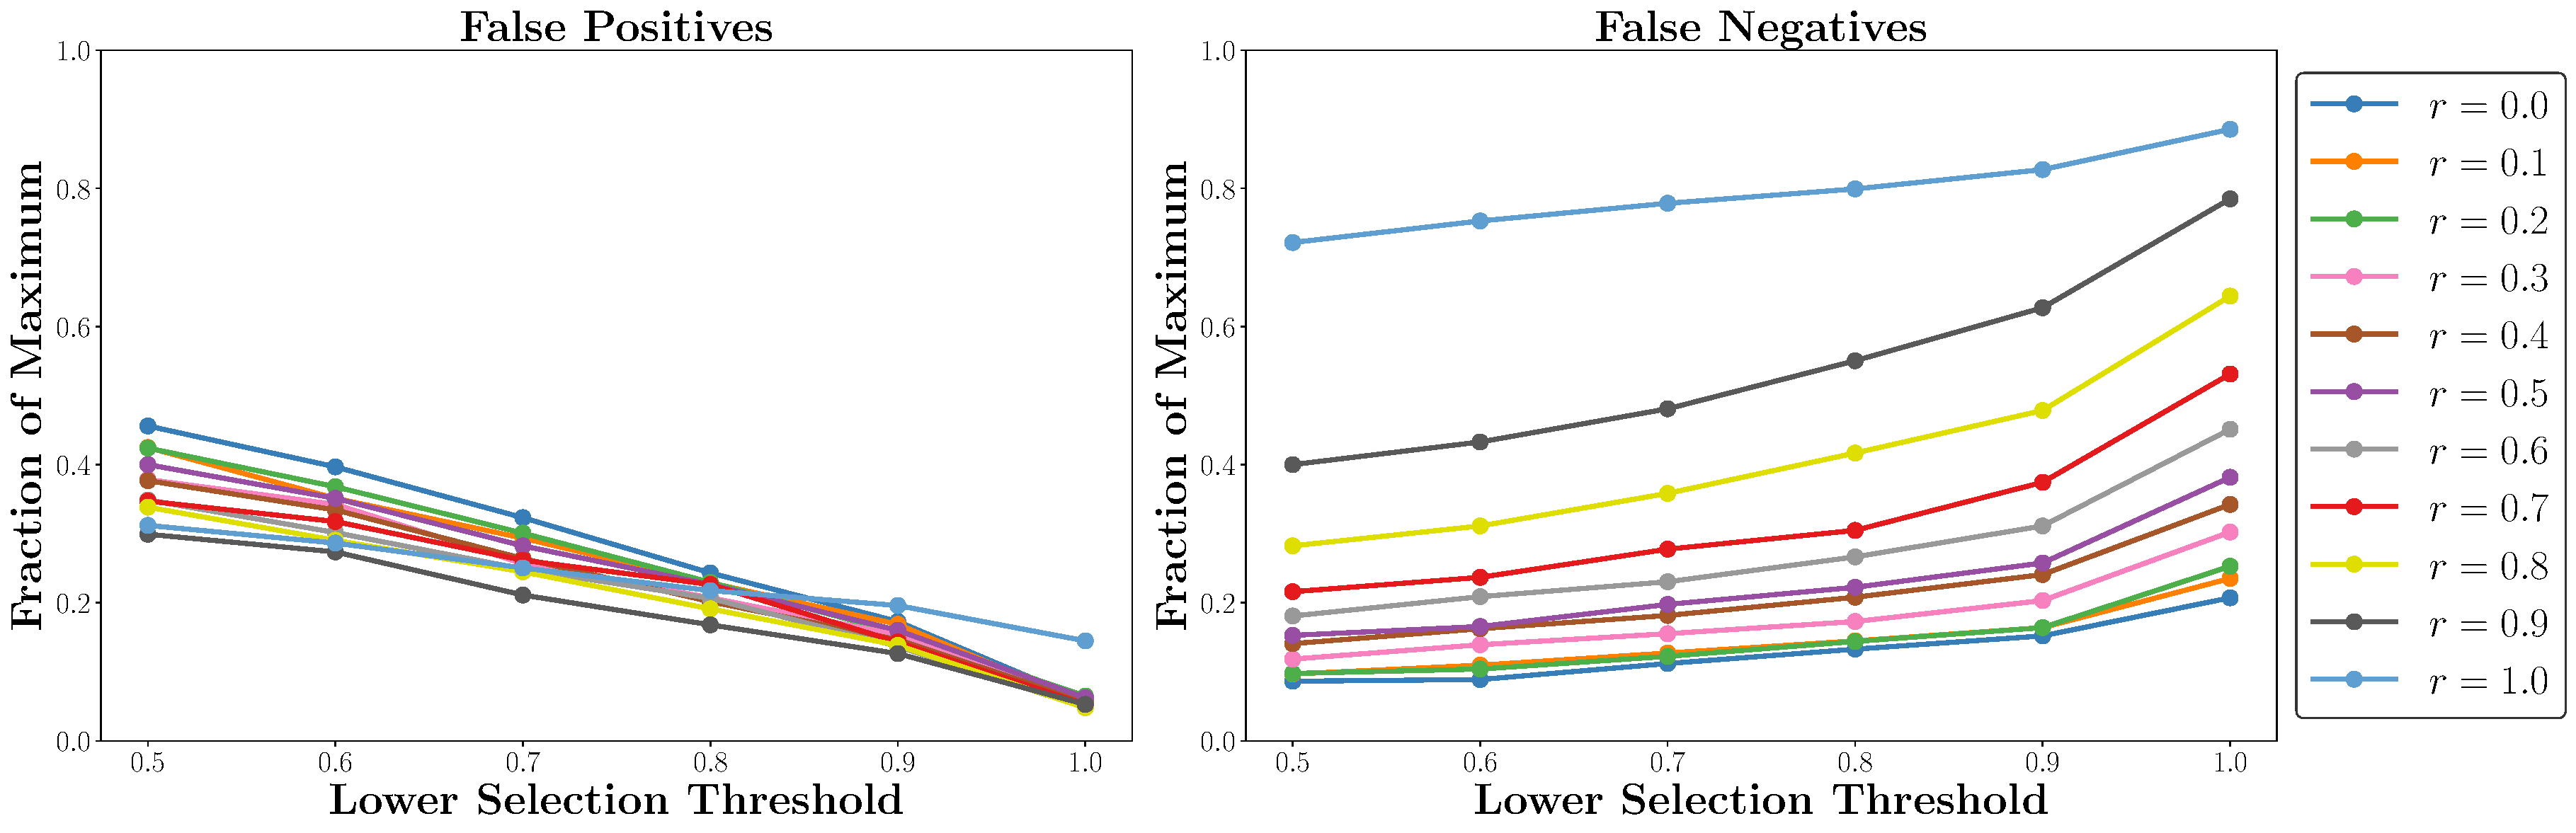
\includegraphics{img/exp2-05.pdf}}
\end{figure}
\begin{figure}[ht]
	\centering
	\scalebox{0.27}{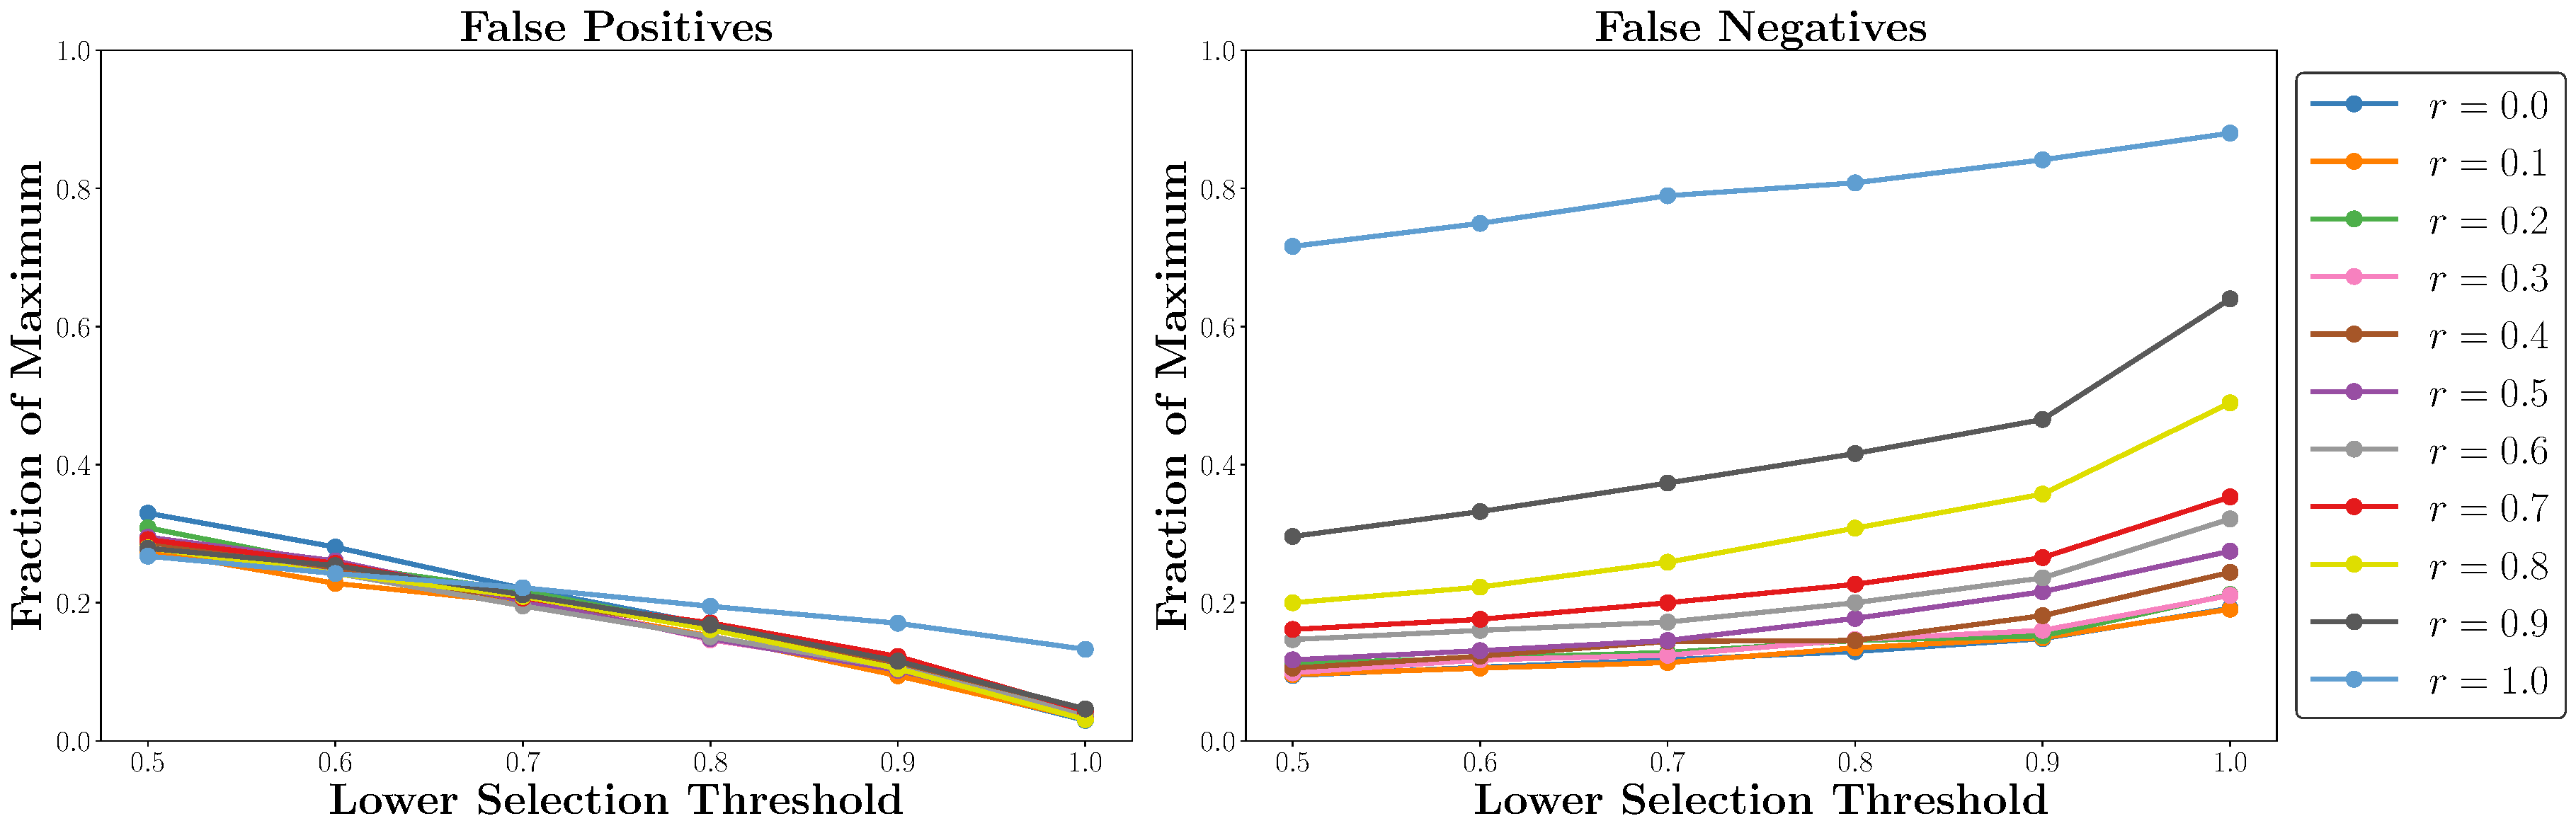
\includegraphics{img/exp2-03.pdf}}
\end{figure}
\begin{figure}[ht]
	\centering
	\scalebox{0.27}{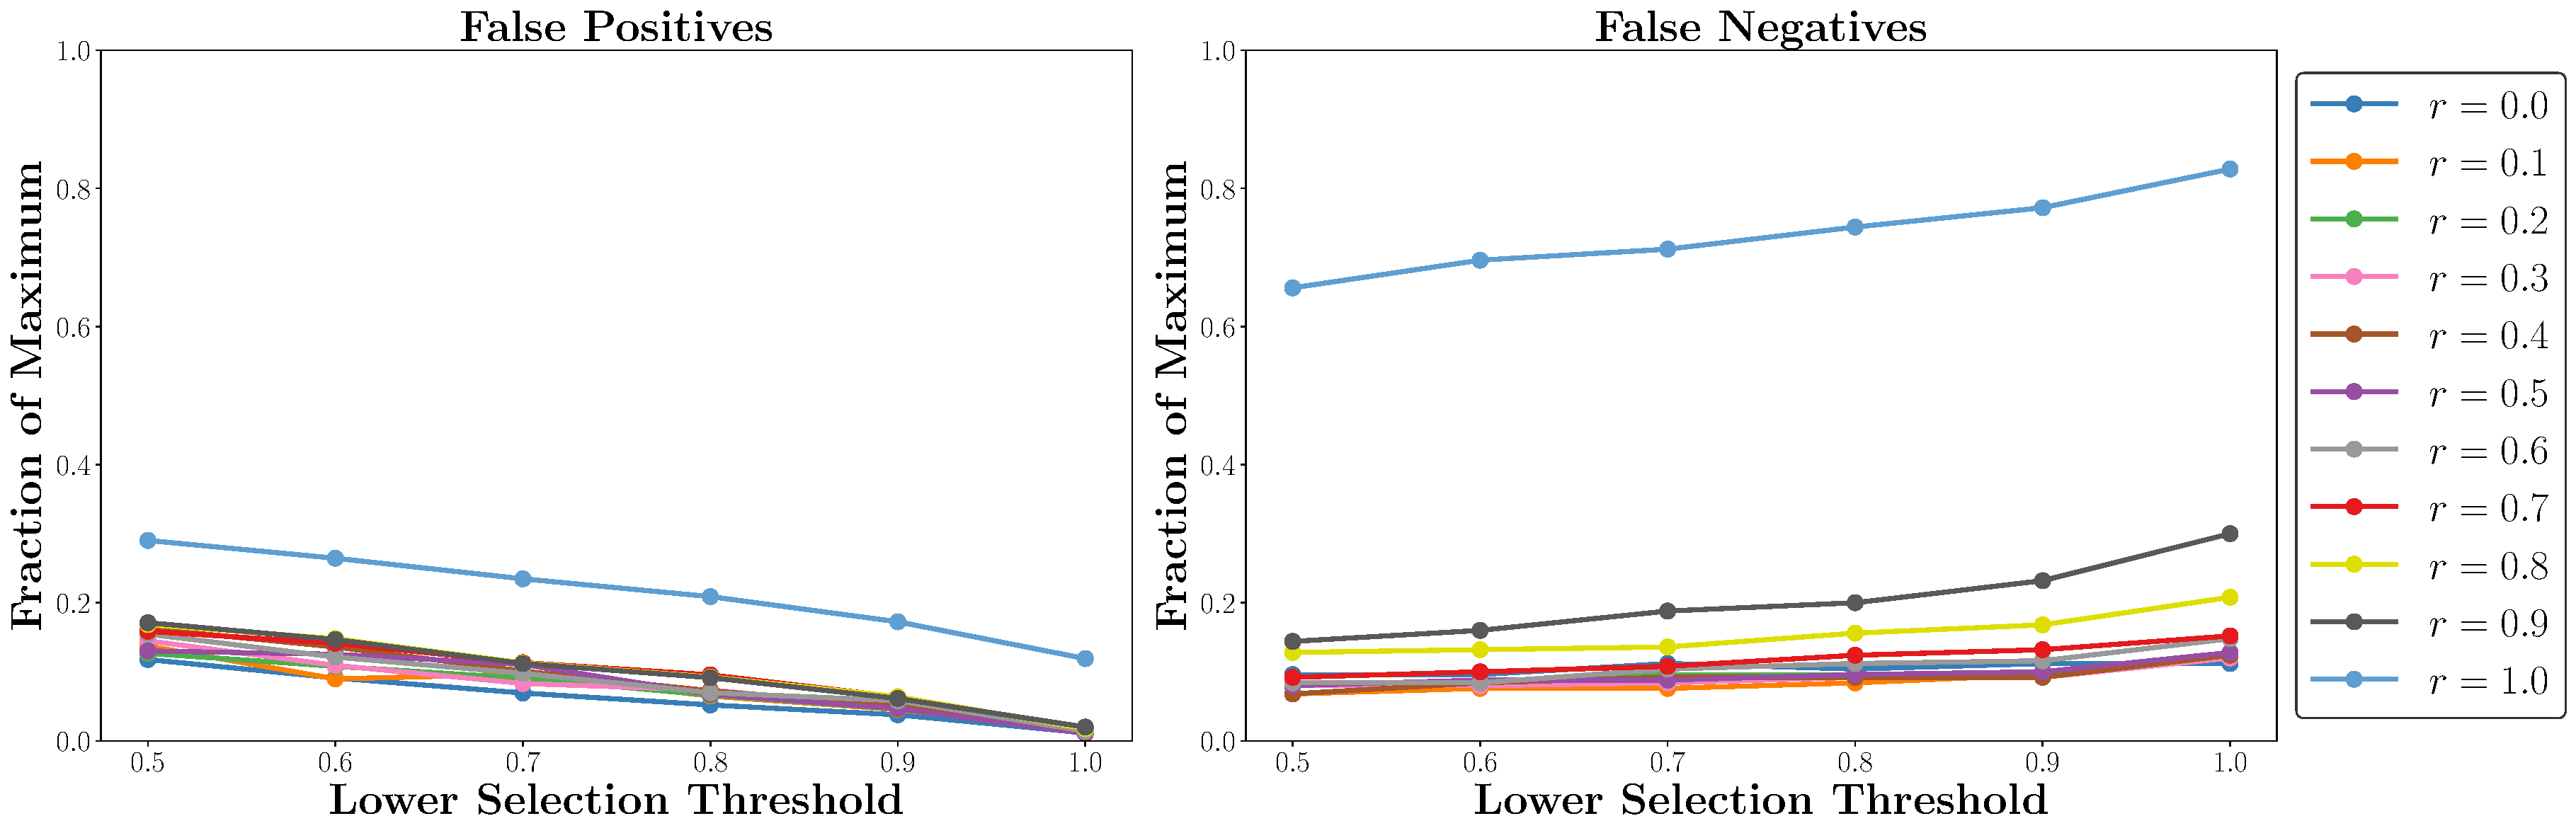
\includegraphics{img/exp2-01.pdf}}
\end{figure}

We also plot selection accuracies below. 

\begin{figure}[ht]
	\centering
	\scalebox{0.35}{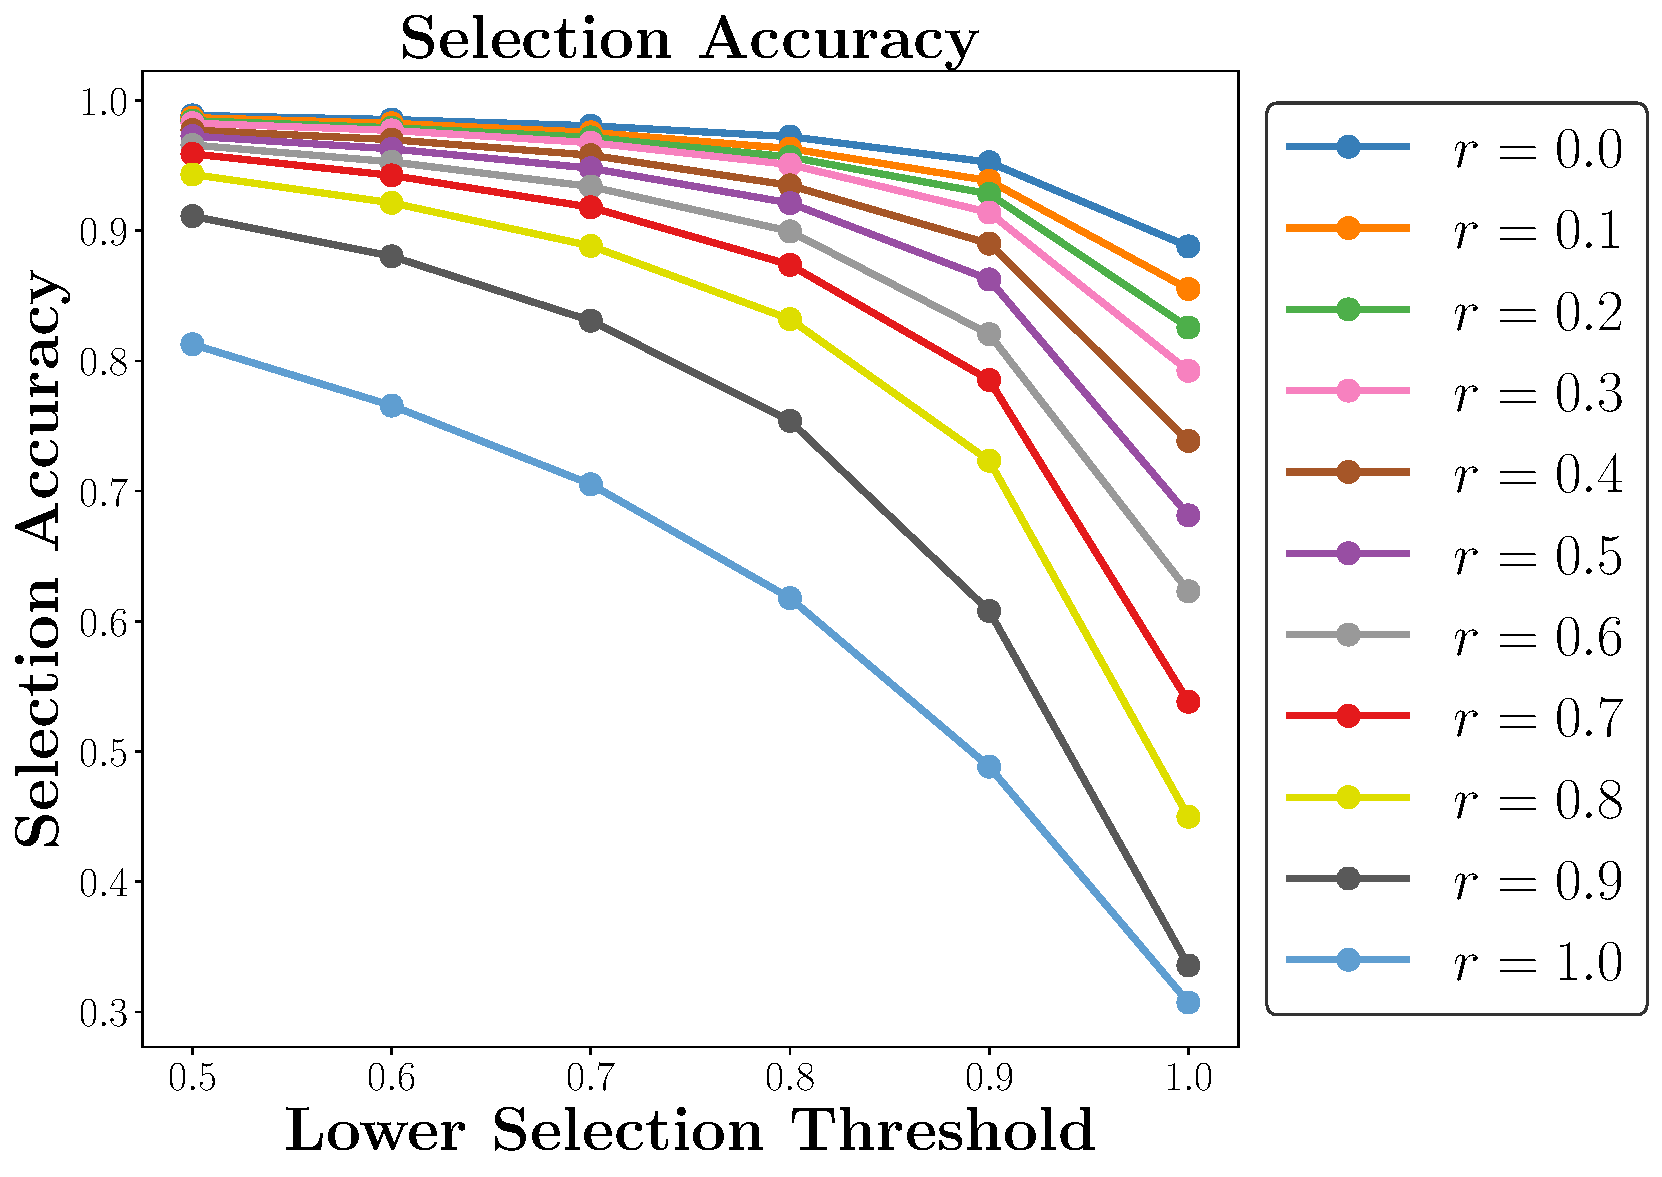
\includegraphics{img/exp2-09-selacc.pdf}}
\end{figure}
\begin{figure}[ht]
	\centering
	\scalebox{0.35}{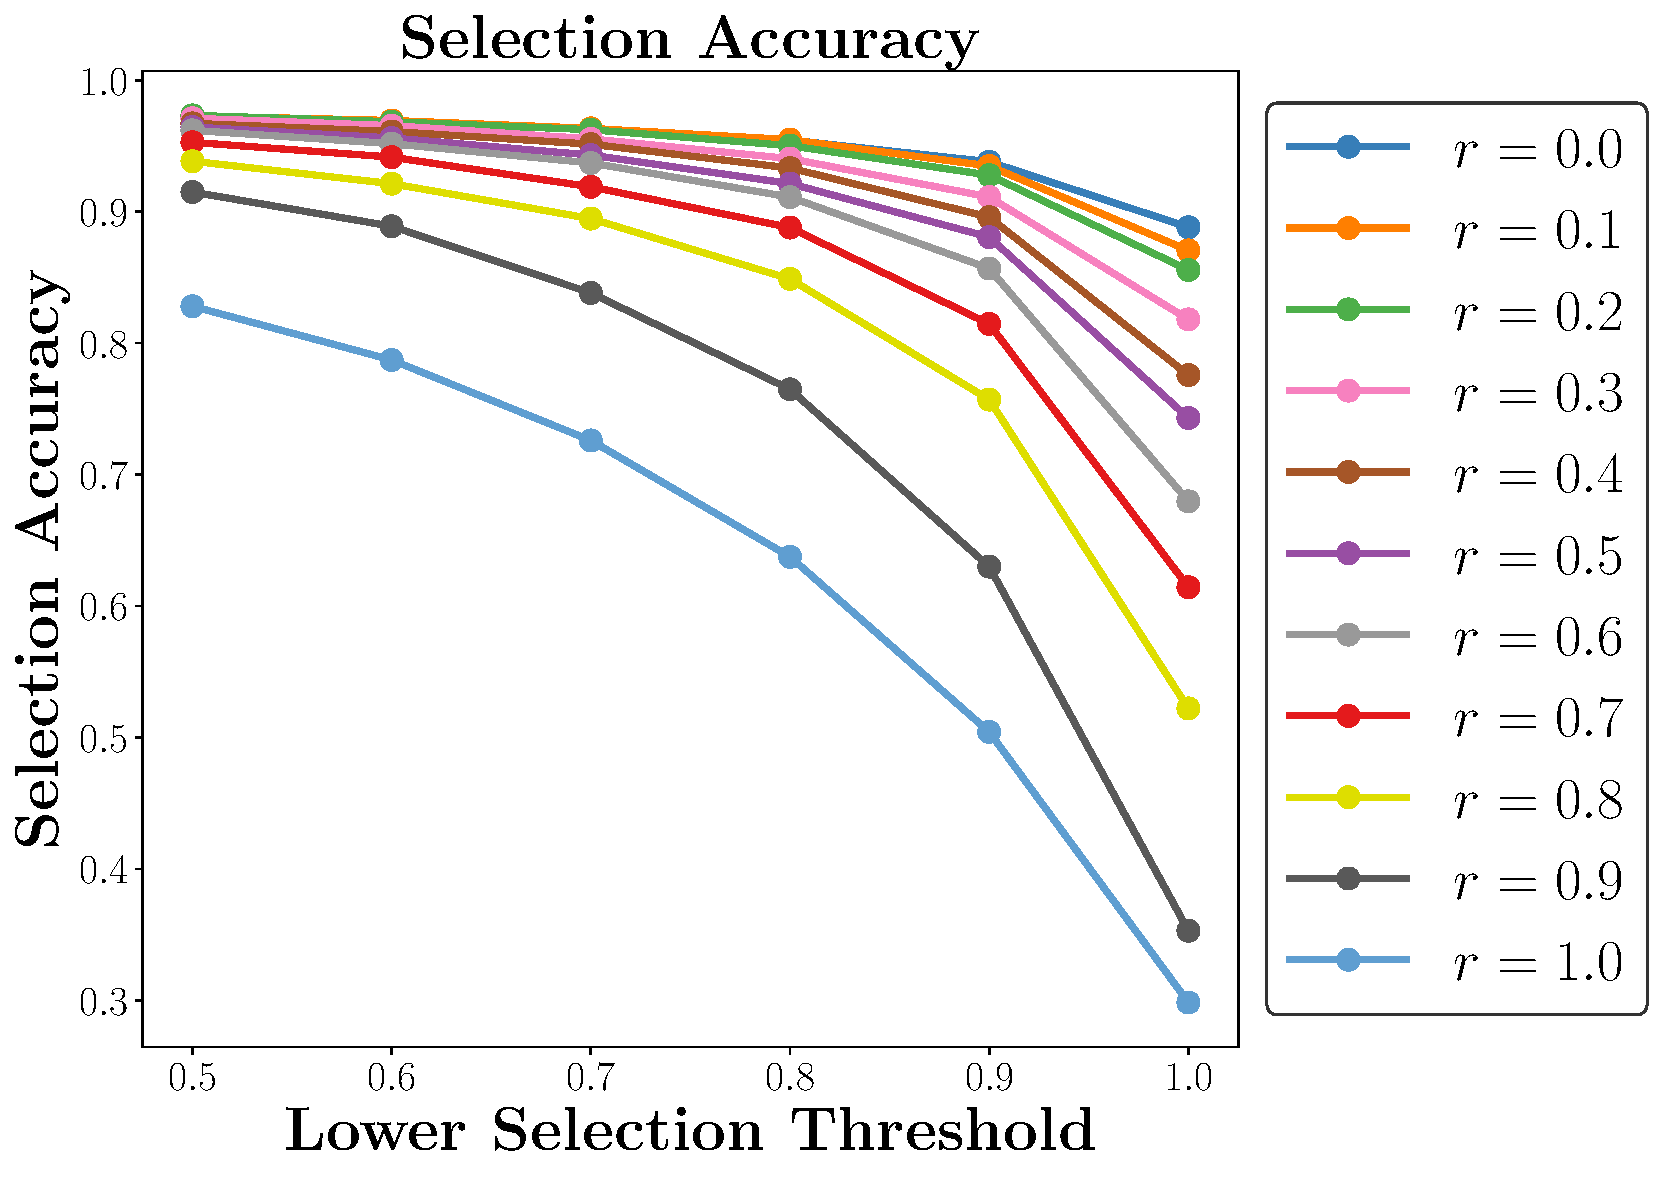
\includegraphics{img/exp2-07-selacc.pdf}}
\end{figure}
\begin{figure}[ht]
	\centering
	\scalebox{0.35}{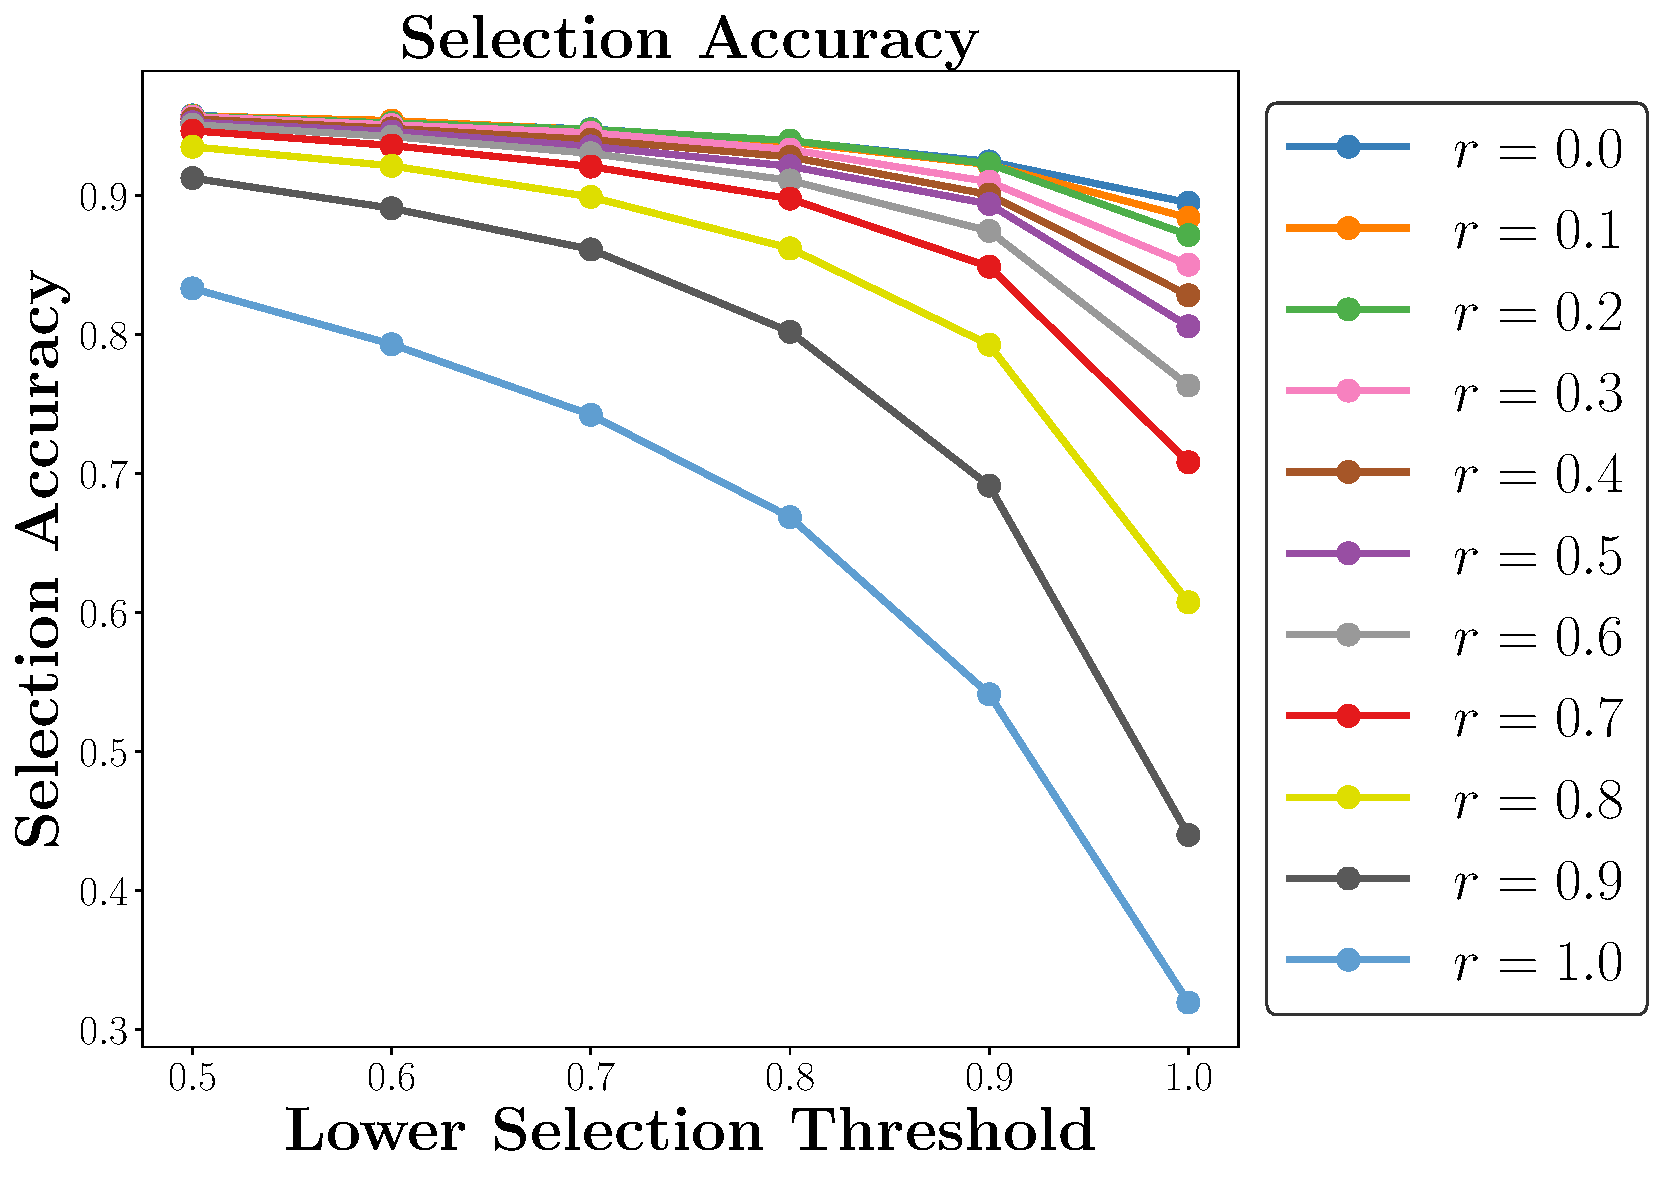
\includegraphics{img/exp2-05-selacc.pdf}}
\end{figure}
\begin{figure}[ht]
	\centering
	\scalebox{0.35}{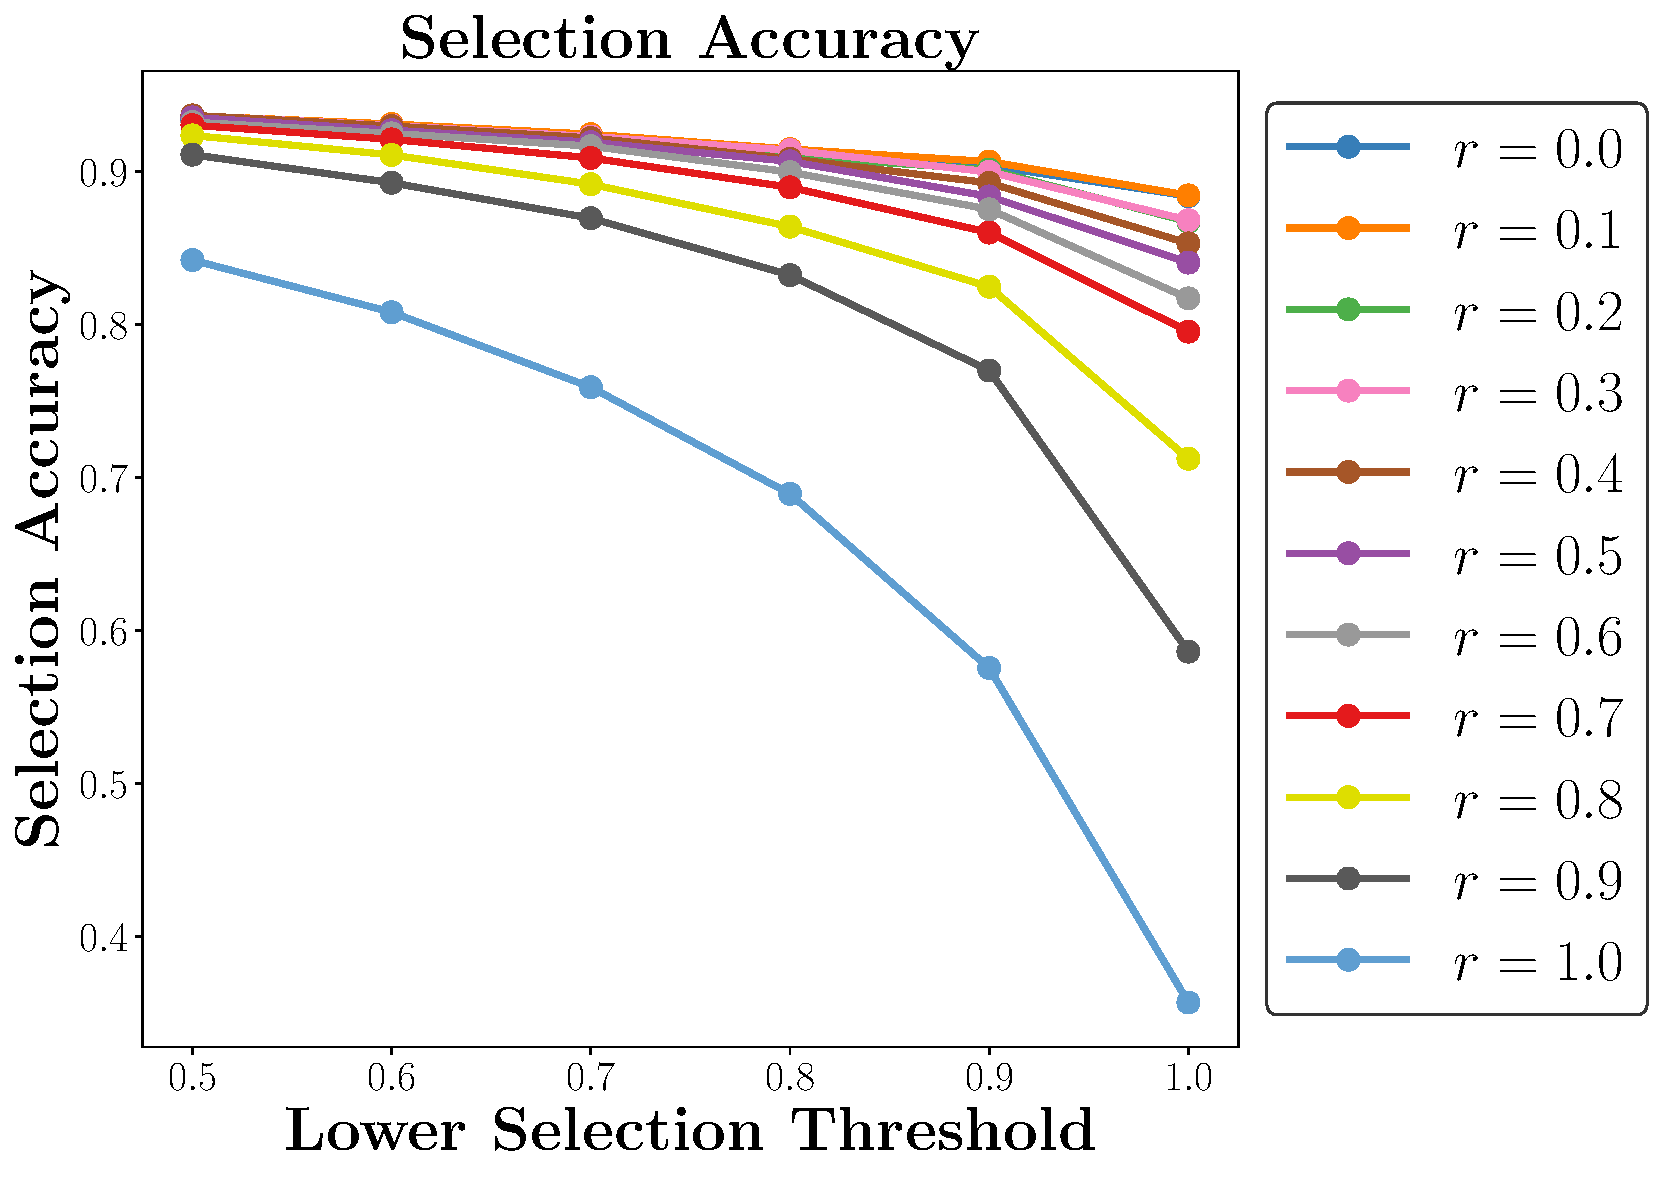
\includegraphics{img/exp2-03-selacc.pdf}}
\end{figure}
\begin{figure}[ht]
	\centering
	\scalebox{0.35}{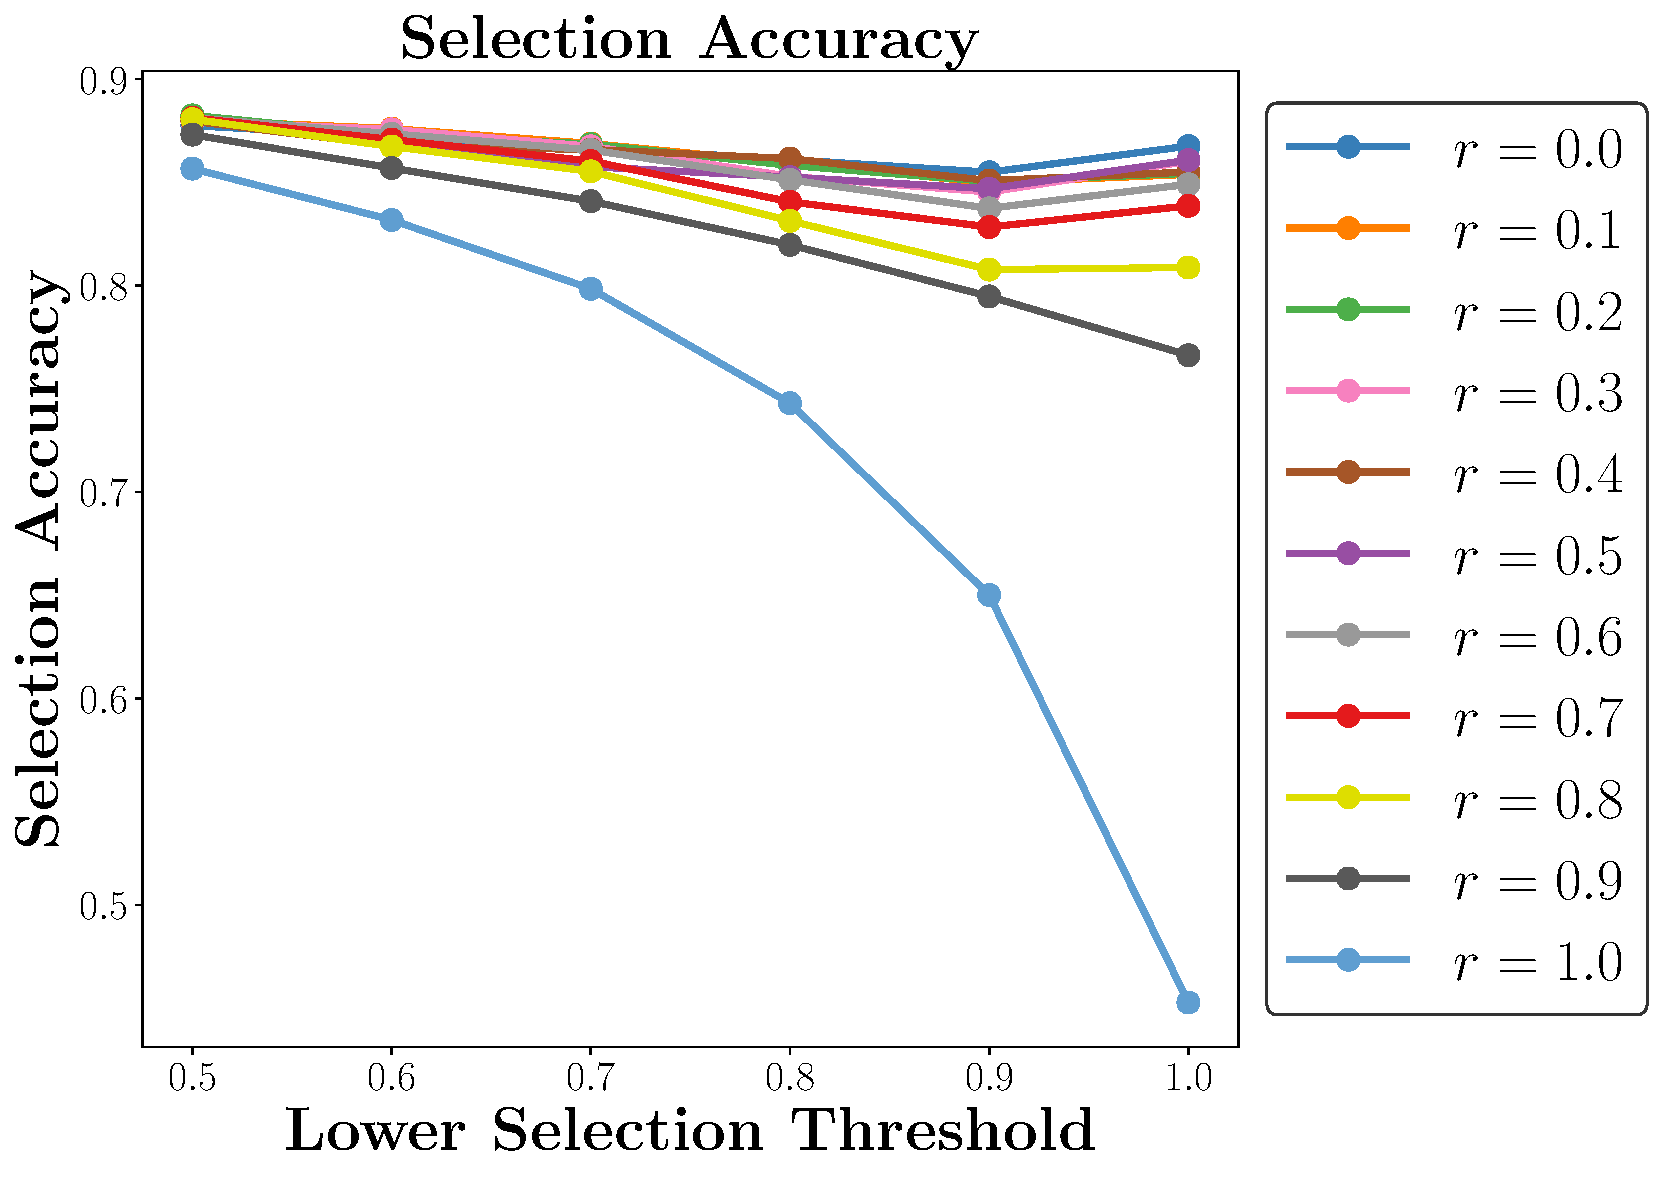
\includegraphics{img/exp2-01-selacc.pdf}}
\end{figure}






\end{document}
